\cleardoublepage
\chapter{Results}
%\label{ch:chapter1}
\label{makereference}
\section{Reconfigurable platform}
La arquitectura descrita en la anterior sección ha sido implementada usando el lenguaje VHDL. Para probar su correcto funcionamiento se ha usado el entorno Vivado y la FPGA Virtex 690T. Si bien no es una FPGA con protección frente a radiación, la arquitectura de este algoritmo es escalable de tal manera que su adaptación a otros tamaños de sensor o FPGAs no debería suponer ningún problema.

\begin{center}
 \begin{tabular}{|c|c|c|c|c|c|} 
 \hline
 Part number & Slices & Logic cells & Flip-Flops & BRAM & DSP Slices \\
 \hline
 XCE7VX690T & 108,300 & 693,120 & 866,400 & 1,470Kb & 3,600\\
 \hline
\end{tabular}
\end{center}

\section{Hyperpectral image datasets}
Para el trabajo se han empleado dos imágenes hiperespectrales, una tomada por el sensor HYDICE y otra por el sensor AVIRIS. Ambas imágenes son usadas comúnmente como referente en aplicaciones hiperespectrales. 
\\
En el terreno de la escena capturada por HYDICE fueron colocados 15 paneles de distinto tamaño en una configuración de 3 x 5. En las siguientes imágenes se puede observar la imagen en falso color y la ubicación de los paneles como ha sido detectada por un software comercial.
\begin{figure}[!ht]
    \begin{tabular}[b]{c|c}\hline
      Horizontal res & 64 \\ \hline
      Vertical res & 64 \\ \hline
      Bands & 210 \\ \hline
      Spectral res & 400 - 2500nm \\ \hline
      Spatial res & 1,56meter/pixel \\ \hline
      Size & 1,6 MB\\ \hline
    \end{tabular}
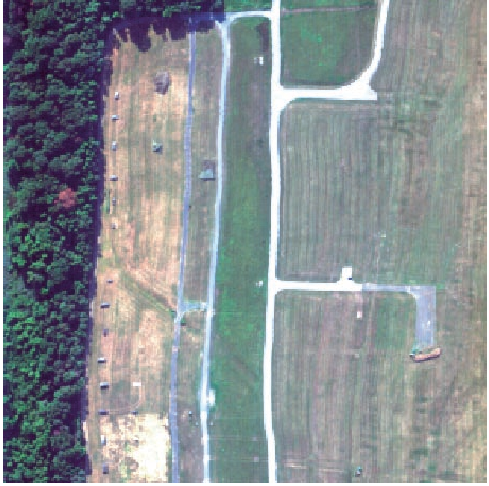
\includegraphics[height=1.5in]{figures/hydice_bad.png}
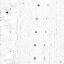
\includegraphics[height=1.5in]{figures/hydice_rx.png}
    \caption{Hydice sensor information and image in false color}
  \end{figure}
  %https://www.indexdatabase.de/db/s-single.php?id=84
\\
\\
La imagen tomada por el sensor AVIRIS fue tomada el 16 de septiembre de 2001, cinco días después de los ataques terroristas que derrumbaron las torres del WTC y sus edificios colindantes. La resolución espacial de esta imagen es muy alta ya que se realizó un vuelo a muy baja altura. Junto a la imagen en falso color se proporciona una imagen con las anomalías detectadas por un programa comercial rodeadas a su vez para indicar su posición.
\begin{figure}[!ht]
    \begin{tabular}[b]{c|c}\hline
      Horizontal res & 614 \\ \hline
      Vertical res & 512 \\ \hline
      Bands & 224 \\ \hline
      Spectral res & 360 - 2500nm \\ \hline
      Spatial res & 1,7meter/pixel \\ \hline
      Size & 140 MB\\ \hline
    \end{tabular}
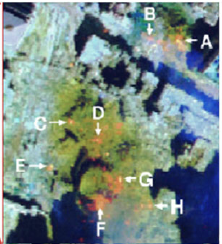
\includegraphics[height=1.5in]{figures/wtc_bad.png}
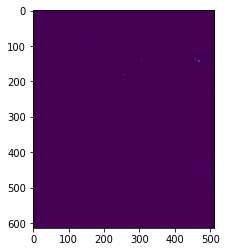
\includegraphics[height=1.5in]{figures/wtc_rx.png}
    \caption{Aviris sensor sensor information and image in false color}
  \end{figure}
  %https://www.indexdatabase.de/db/s-single.php?id=28
\\
\\
\section{Adequacy of approximation}
\subsection{Floating point}
Los resultados proporcionados por la versión en punto flotante de este sistema son los mismos que los proporcionados por la versión en software equivalente, por lo que esta se puede dar por válida.

\subsection{Fixed point}
La versión en punto fijo del sistema es una aproximación al sistema en punto flotante con la intención de mantener la mayor precisión posible con un uso limitado de recursos.
Por tanto, los resultados son diferentes y hay que realizar una valoración sobre su precisión. Para ello, se han utilizado 3 métricas.
\\
\\
En la primera y más simple, se ha comprobado que cantidad de anomalías detectadas se pueden encontrar en las primeras x posiciones en ambos resultados, sin importar el orden.
\\
\\
Ampliando la anterior estrategia, se ha comprobado para los elementos no coincidentes, si se ha detectado algún vecino en el entorno. Un vecino es definido como un pixel adyacente, tanto en linea recta como en diagonal.
\\
\\
Para terminar se ha vuelto a extender la primera estrategia, esta vez se ha comprobado si para los no coincidentes se ha encontrado una anomalía con una similaridad espectral menor de 5 grados.
\\
%https://www.harrisgeospatial.com/docs/SpectralAngleMapper.html
El Mapeador de Ángulos Espectrales (SAM) es una clasificación espectral basada en la física que utiliza un ángulo n-D para hacer coincidir los píxeles con los espectros de referencia. El algoritmo determina la similitud espectral entre dos espectros calculando el ángulo entre los espectros y tratándolos como vectores en un espacio con una dimensionalidad igual al número de bandas. Esta técnica, cuando se utiliza en los datos de reflectancia calibrados, es relativamente insensible a los efectos de la iluminación y del albedo
\begin{figure}[h!]
\begin{minipage}[t]{0.5\linewidth}
\centering
\[\alpha = \cos^{-1}\left ( \frac{\sum\limits^{nb}_{i=1}{t_{i}r_{i}}}{\left ( \sum\limits^{nb}_{i=1}{t_{i}^2} \right )^{1/2}\left ( \sum\limits^{nb}_{i=1}{r_{i}^2} \right )^{1/2}} \right )\]
\label{sam}
\end{minipage}
\begin{minipage}[t]{0.05\linewidth}
\end{minipage}
\begin{minipage}[t]{0.45\linewidth}
\vspace{0.7cm}
$\alpha$ = spectral angle between vectors
\\
nb = number of spectral bands
\\
t = target pixel
\\
r = reference pixel
\end{minipage}
\caption{Spectral Angle Mapper algorithm.}
\end{figure}

En los resultados de HYDICE se puede apreciar como si un pixel no es el detectado, tampoco lo es un pixel vecino, pero que todos los resultados concuerdan según su firma espectral. Esto es a causa del gran tamaño de los targets a detectar, donde existen varios pixeles en el mismo target y el orden de detección puede variar. Sin embargo, al ser todos los targets similares espectralemente, la firma siempre concuerda. La imagen resulta por lo tanto bastante fácil de analizar y se han logrado buenos resultados.
\begin{figure}[!ht]
	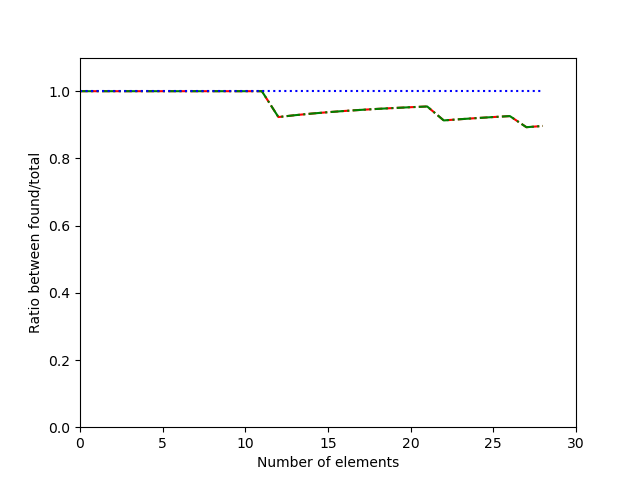
\includegraphics[height=2.0in]{figures/hydice.png}
	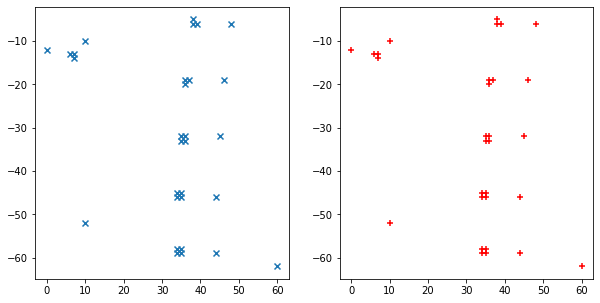
\includegraphics[height=2.0in]{figures/hydice_res.png}
\end{figure}

La imagen del WTC es sim embargo más compleja, y se puede observar que la detección de pixeles exactos y vecinos falla. Sin embargo, las firmas espectrales concuerdan en su mayor parte, sobretodo teniendo en cuenta el número de hot spots reales encontrados en la imagen. Por lo tanto os resultados se pueden tomar también como exitosos.
\begin{figure}[!ht]
	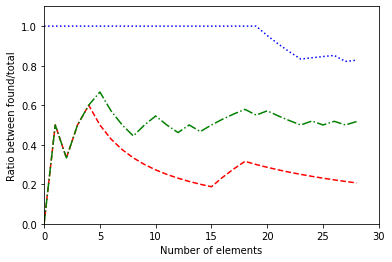
\includegraphics[height=2.0in]{figures/wtc.png}
	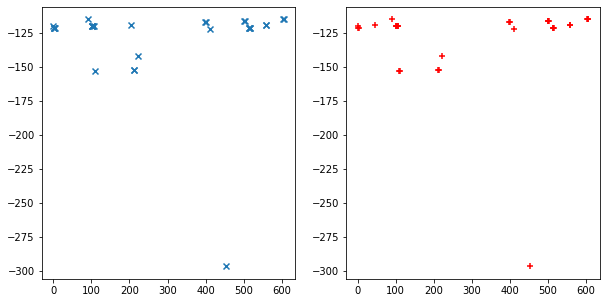
\includegraphics[height=2.0in]{figures/wtc_res.png}
\end{figure}

Cabe destacar que los valores de desplazamiento dentro de los cálculos han sido adaptados para cada imagen con la intención de detectar el mayor número de anomalías posibles, por lo que los resultados obtenidos en un sistema real serán ligeramente menores. Aún así, los valores entre las dos imágenes son bastante similares, pese a la gran diferencia entre los datos que representan.
\\
Además, puesto que se trata de un sistema reconfigurable, estos valores pueden ser modificados después de la puesta en marcha del sistema, tanto para aceptar un mayor rango de imágenes, como para obtener resultados más exactos.

nota: tengo que incluir una leyenda
nota: tengo que pintar bien las imágenes para averigüar que estoy analizando realmente y poder hacer una mejor valoración de los resultados

\section{Computational efficiency}
A la hora de evaluar el rendimiento hay que evaluar tanto los recursos usados como el tiempo de procesamiento. Estos datos se dan tanto en los obtenidos para los dos sensores como en función de sus características, más específicamente número de bandas y de pixeles.
\\
Cabe destacar que los datos de rendimiento se han obtenido ignorando la entrada y salida de los datos, que es frecuentemente el cuello de botella en este tipo de sistemas.
\\

También se ofrece una comparación del gasto de recursos por módulo, que se encuentra estrechamente relacionado con su complejidad en tiempo

\begin{center}
 \begin{tabular}{|c|c|c|c|c|} 
 \hline
 Module & LUT & Register & BRAM & DSP \\ [0.5ex] 
 \hline\hline
 Inverse & $410*bands+3484$ & $316*bands+10427$ & $<bands$ & $10*bands$\\ 
 \hline
 Mean subtraction & $bands+41$ & $136$ & $0$ & $1$\\ 
 \hline
 Matrix multiplication & $80*bands+75$ & $91*bands+223$ & $pixels/64$ & $4*bands$\\ 
 \hline
 Sort results & $186$ & $176$ & $0$ & $0$\\ 
 \hline
\end{tabular}
\end{center}

\begin{center}
 \begin{tabular}{|c|c|} 
 \hline
 Stage & Latency \\ [0.5ex] 
 \hline\hline
 Inverse & $\mathcal{O}(bands+bands^2) = \mathcal{O}(bands^2)$\\ 
 \hline
 Mean subtraction & $\mathcal{O}(1)$\\
 \hline
 Matrix multiplication & $\mathcal{O}(bands*pixels+bands)$\\
 \hline
 Sort results & $\mathcal{O}(2*bands) = \mathcal{O}(bands)$\\
 \hline
\end{tabular}
\end{center}

Nota: aquí me falta alguna cosilla.
Finalmente también se proporciona el gasto total de recursos proporcionado por Vivado y las especificaciones de tiempo y frecuencias
\begin{center}
 \begin{tabular}{|c|c|c|c|c|} 
 \hline
 Resource & Hydice & Aviris\\ [0.5ex] 
 \hline\hline
 periodo & 0 & 0\\ 
 \hline
 frecuencia & 0 & 0\\ 
 \hline
 setup & 0 & 0\\ 
 \hline
 hold & 0 & 0\\ 
 \hline
\end{tabular}
\end{center}